\chapter{Análise Bibliográfica sobre Quantum Key Distribution(QKD) Na Segurança Computacional, por Rafael Nogalha\label{chap:bibliometria:rafaelnogalha}}

\section{Planejamento do estudo}

Com o crescimento do número de ataques cibernéticos a empresas governamentais e grandes corporações no mundo todo, o estudo e investimento por formas mais seguras de criptografia se tornou prioridade em diversas entidades. 

Dessa forma, com o aumento exponencial de informação produzida no mundo (\textit{BigData}), houve uma expansão no uso de tecnologias quânticas para o fim de segurança computacional, tendo em vista que a matemática computacional convencional não é capaz de ser escalável em relação a quantidade de informação produzida e assim não é mais segura também.. Assim, o investimento está sendo feito em \textit{Distribuição de chave quântica} ou QKD, pois o poder do processador quântico e a escalabilidade são praticamente infinitos comparados à computação tradicional, além de oferecer uma segurança computacional dupla, na qual é praticamente impossível de ser quebrada até mesmo por computadores quânticos. Assim, a presente análise busca evidenciar aspectos a respeito da produção científica sobre esse tema. Os pontos de pesquisa são:

\begin{itemize}
    \item Como a produção científica em relação à QKD evoluiu nos últimos anos?
    \item Quais são as principais definições e campos relacionados à QKD?
    \item Os países têm feito um \textit{coworking} em relação ao tema?
\end{itemize}

\subsection{Uso do Bibliometrix e Biblioshiny}

A ferramenta que será utilizada para análise e filtragem dos dados será a \textit{Bibliometrix}, juntamente com a interface \textit{Biblioshiny}, para gerar gráficos e grafos iterativos, todos eles personalizáveis, auxiliando na análise dos dados referente ao assunto tratado no presente artigo.

\section{Coleta de dados}

A coleta de dados foi feita pelo Web of Science (WeS) no dia 8 de Fevereiro de 2022, com acesso feito por meio do Periódicos Capes disponibilizado por meio da matrícula da Universidade de Brasília (UNB).Foram feitas buscas na coleção \textit{Science Citation Index Expanded (SCI-EXPANDED)} que foca mais na área das ciências exatas e naturais. 

\subsection{Query de Busca}

A \textit{query} de busca pode ser acessada na seguinte listagem de código \ref{rafael-nogalha:query}

\lstinputlisting[numbers=left,basicstyle=\normalsize\ttfamily,caption={\query\ de busca sobre Mineração de Dados Educacionais.},label=rafael-nogalha:query]
{experiments/rafaelnogalha/PesquisaBibliografica/query/query-de-busca.txt}

No primeiro momento, foi feita uma pesquisa com os seguintes termos "quantum key distribution (Topic)", entretanto isso resultou em muitos artigos que abordavam aspectos somentes físicos do QKD, e o foco da pesquisa é uma análise estatística sobre a influência da QKD na segurança computacional. Dessa forma, adicionou-se na \textit{query} de busca as seguintes cláusulas "(experimental  or statist* and security)", resultando assim em 1.450 resultados na WeS. Essa base de dados está presente \href{https://github.com/jhcf/Comput-Experim-20212/tree/main/experiments/rafael-nogalha/PesquisaBibliografica/QKDSegurancaComputacional/dataset/dataset.txt}{no seguinte link}. A exportação foi feita com a opção "Plain text file" na opção em inglês e "Exportar arquivo de texto sem formatação" na opção em português. A seleção personalizada foi feita com todas as 29 opções possíveis e os registros foram extraídos em um intervalo de 1000 e 1000 e depois foram concatenados de forma manual.

\subsection{Filtragem dos dados}

após a exportação do \textit{dataset}, foram considerados os artigos ciêntíficos publicados em periódicos, artigos de anais de congresso e artigos de acesso antecipado. Dessa forma, restaram 1.148   registros para análise. Assim, esse novo \textit{dataset} será chamado de @QKD-rafael-nogalha.

\section{Análise dos dados}

\subsection{Análise descritiva}

Usando o bibliometrix e a interface biblioshiny, é possível obter as principais informações em relação ao \textit{dataset} @QKD-rafael-nogalha, seguem abaixo essas informações:
\begin{description}
    \item[\textbf{Timespan}] os artigos do \textit{dataset} @QKD-rafael-nogalha estão presentes no intervalo de 1991 a 2022.
    Assim, é possível afirmar que o tema é muito novo, tendo em vista que antes dos anos 1991 não foi publicado nenhum artigo se referindo ao tema.
    \item[\textbf{Sources (Journals, Books, etc)}] há 259 fontes de informação no \textit{dataset} @QKD-rafael-nogalha.
    \item[\textbf{Documents}] há 1148 documentos no \textit{dataset} @QKD-rafael-nogalha.
    \item[\textbf{Average years from publication}] a média de anos de publicação do \textit{dataset} @QKD-rafael-nogalha é 7.65.
    \item[\textbf{Average citations per documents}] a média de citações por documento é de 39.39 no \textit{dataset} @QKD-rafael-nogalha.
    \item[\textbf{Average citations per year per doc}] a média de citações por ano por documento é de 3.744 no \textit{dataset} @QKD-rafael-nogalha.
    \item[\textbf{References}] há 24471 referências no \textit{dataset} @QKD-rafael-nogalha.
    \item[\textbf{article}] há 1123 artigos no \textit{dataset} @QKD-rafael-nogalha.
    \item[\textbf{article; proceedings paper}] há 25 artigos de anais de congresso no \textit{dataset} @QKD-rafael-nogalha.
    \item[\textbf{Keywords Plus (ID)}] há 1783 Keywords Plus (ID) no \textit{dataset} @QKD-rafael-nogalha.
    \item[\textbf{Author's Keywords (DE)}] há 1200 palavras-chave que foram adicionadas pelos autores no \textit{dataset} @QKD-rafael-nogalhao.
    \item[\textbf{Authors}] há 3614 nomes de autores distintos no \textit{dataset} @QKD-rafael-nogalha
    \item[\textbf{Author Appearances}] os 6292 autores distintos aparecem no \textit{dataset} @QKD-rafael-nogalha.
    \item[\textbf{Authors of single-authored documents}] 40 autores publicaram artigos sem co-autores no \textit{dataset} @QKD-rafael-nogalha.
    \item[\textbf{Authors of multi-authored documents}] 3574 autores foram autores de artigos em conjunto com outros autores no \textit{dataset} @QKD-rafael-nogalha.
    \item[\textbf{Single-authored documents}] 50 artigos foram escritos por um único autor no \textit{dataset} @QKD-rafael-nogalha.
    \item[\textbf{Documents per Author}] a taxa de documentos por autor é de 0.318 no \textit{dataset} @QKD-rafael-nogalha.
    \item[\textbf{Authors per Document}] a taxa de autor por documento é de 3.15 no \textit{dataset} @QKD-rafael-nogalha.
    \item[\textbf{Co-Authors per Documents}] há em média 5.48 autores por artigos no \textit{dataset} @QKD-rafael-nogalha.
    \item[\textbf{Collaboration Index}] o índice de colaboração é de 3.26 no \textit{dataset} @QKD-rafael-nogalha.
\end{description}

\section{Visualização dos dados}

\subsection{Evolução da produção Científica}

\begin{figure}[H]
    \centering
    \includegraphics[width=1\textwidth]{experiments/rafaelnogalha/PesquisaBibliografica/QKDSegurancaComputacional/images/producao_cientifica_anual.png}
    \caption{Evolução da produção científica anual no \textit{dataset} @QKD-rafael-nogalha.}
    \label{fig:evol:anual:@QKD-rafael-nogalha}
\end{figure}

De acordo com a Figura \ref{fig:evol:anual:@QKD-rafael-nogalha} é possível observar que o crescimento da produção científica no tema está acontecendo de forma exponencial, com uma taxa de 8.57\% ao ano. E especificamente a partir de 2007 foi quando ocorreu um o início do crescimento maior da produção científica em relação ao tema.

\subsection{Citações médias Por Ano}

\begin{figure}[H]
    \centering
    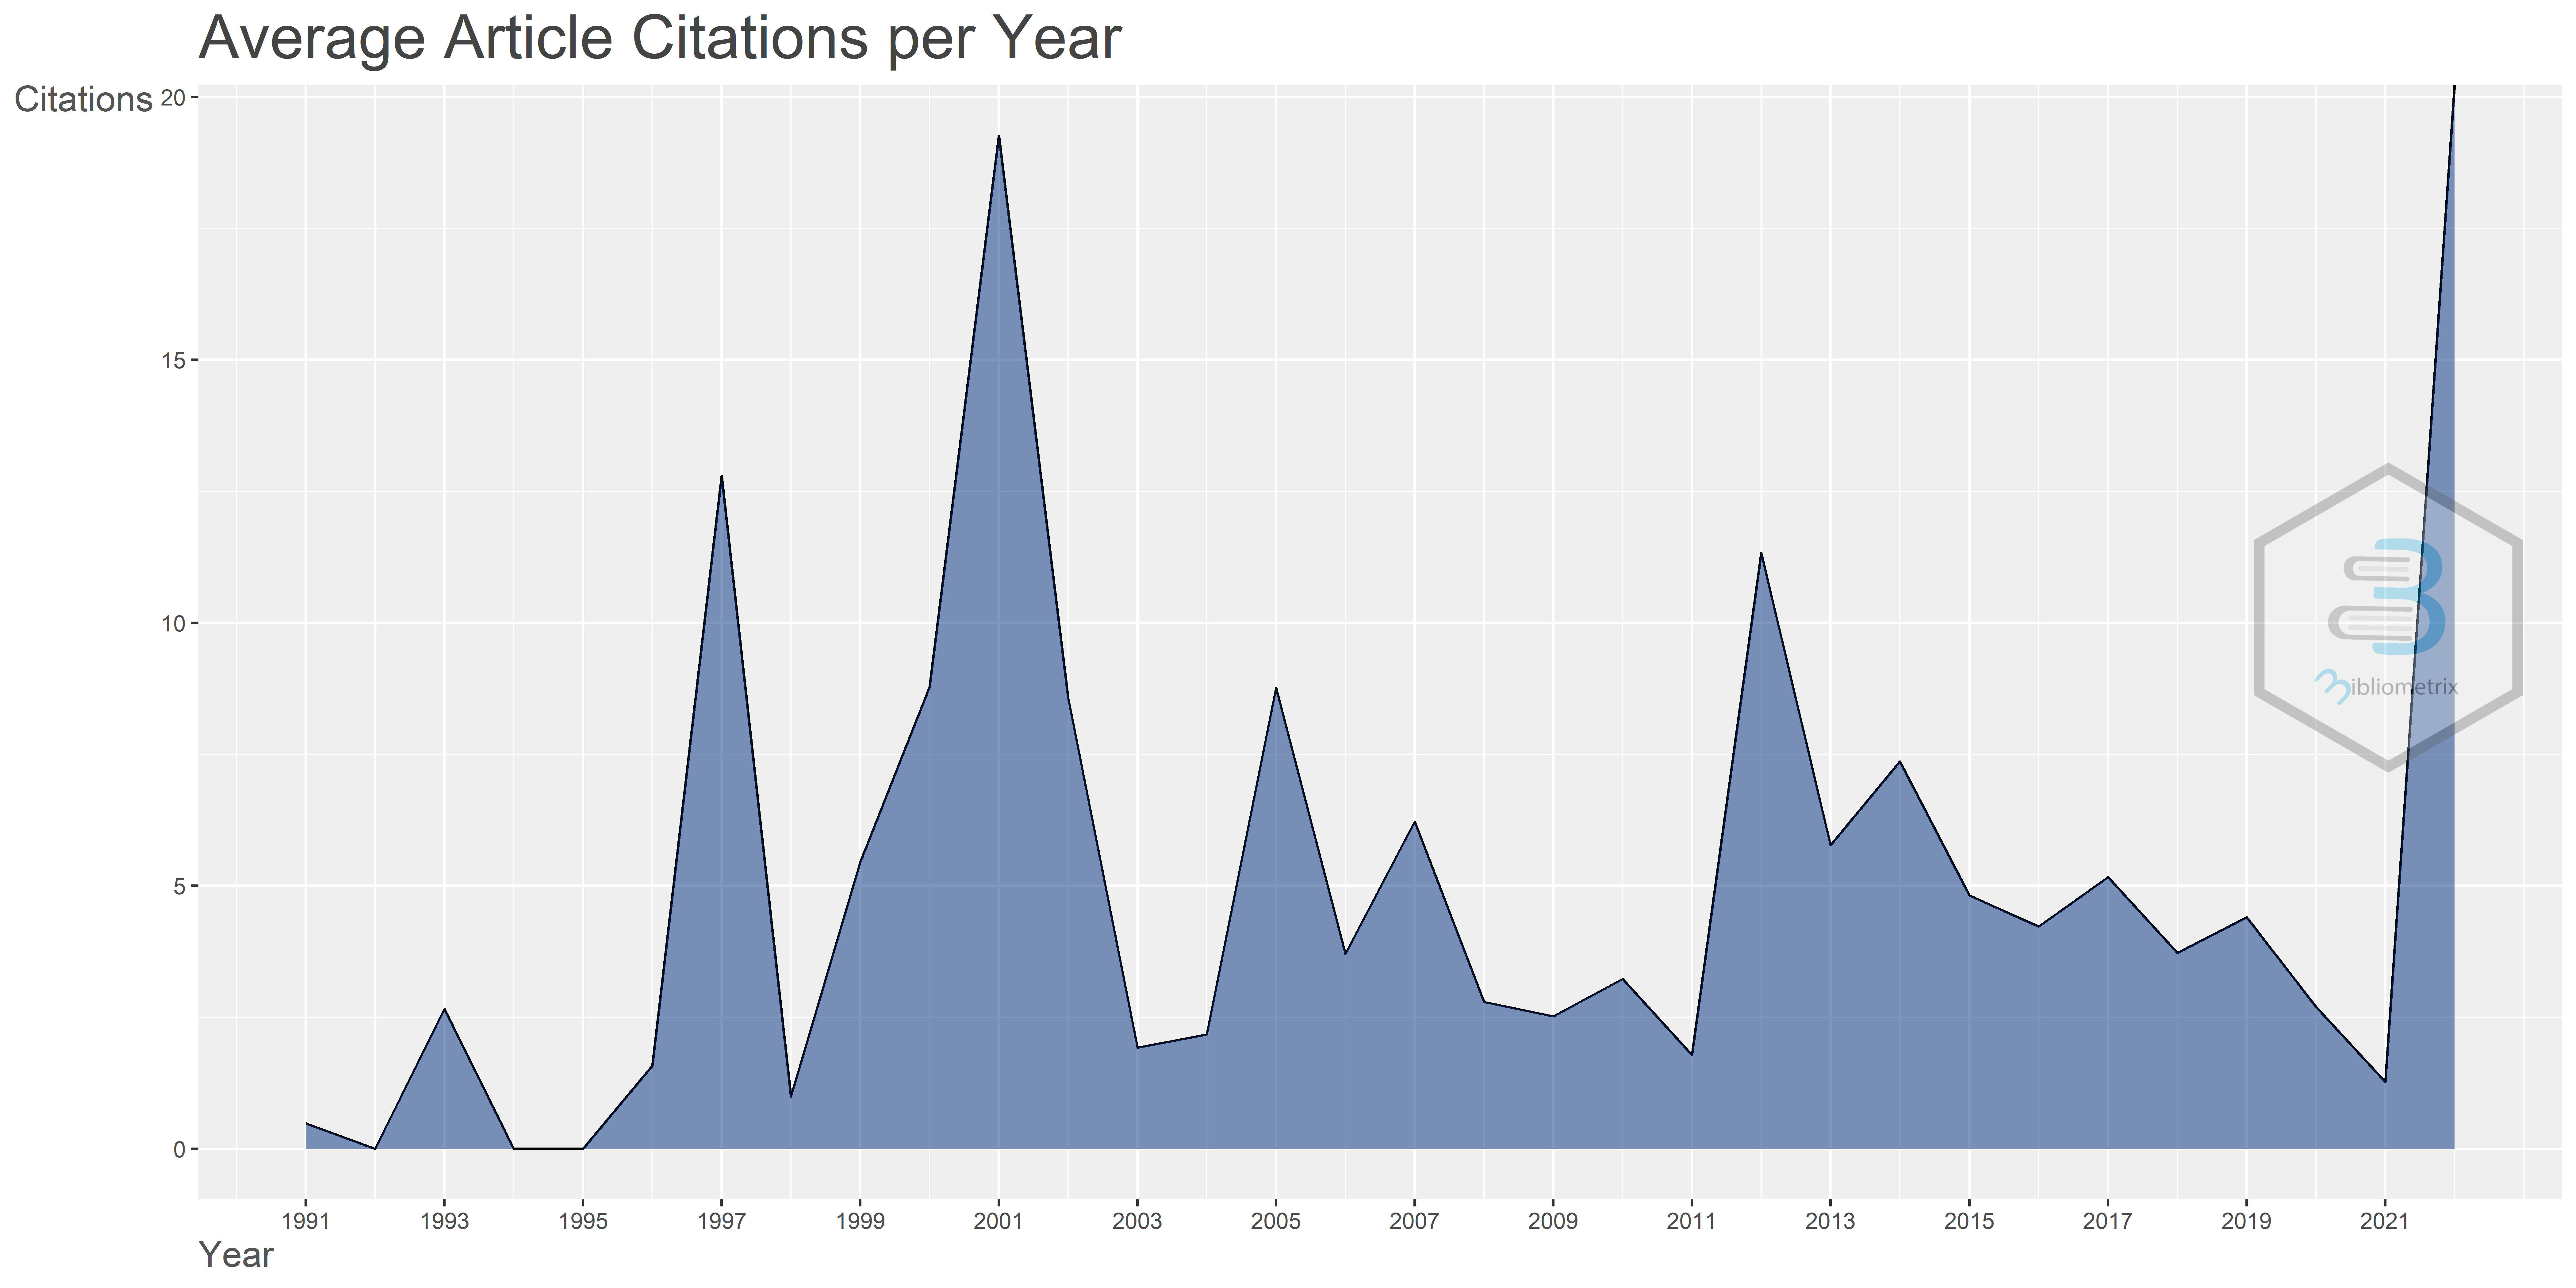
\includegraphics[width=1\textwidth]{experiments/rafaelnogalha/PesquisaBibliografica/QKDSegurancaComputacional/images/citacoes_media_por_ano.png}
    \caption{Citações médias por ano no \textit{dataset} @QKD-rafael-nogalha.}
    \label{fig:citacoes:anual:@QKD-rafael-nogalha}
\end{figure}

É possível observar na figura \ref{fig:citacoes:anual:@QKD-rafael-nogalha} a evolução das citações médias por ano. Observe que nos anos de 1997, 2001 e 2012 tiveram picos de citações.

\subsection{Principais Definições, Campos Relacionados - \textit{Three-Field Plots (Sankey diagram)}}

A análise de estrutura conceitual iniciou-se por meio da geração do mapa fatorial \ref{fig:mapa:fatorial:@QKD-rafael-nogalha}, da análise \textit{tree plot} \ref{fig:three:plot:@QKD-rafael-nogalha} e da tabela de palavras relevantes presentes na figura \ref{fig:campos:plot:@QKD-rafael-nogalha}. Pela análise das figuras é possível observar que as três palavras mais relevantes são: \textbf{cryptography} \textbf{security} e \textbf{key distribution}. Tais palavras estão em concordância com o tema \textit{Quantum Key Distribution(QKD) Na Segurança Computacional} e dão uma compreensão em relação ao conceitos relacionados a tal área.

\begin{figure}[H]
    \centering
    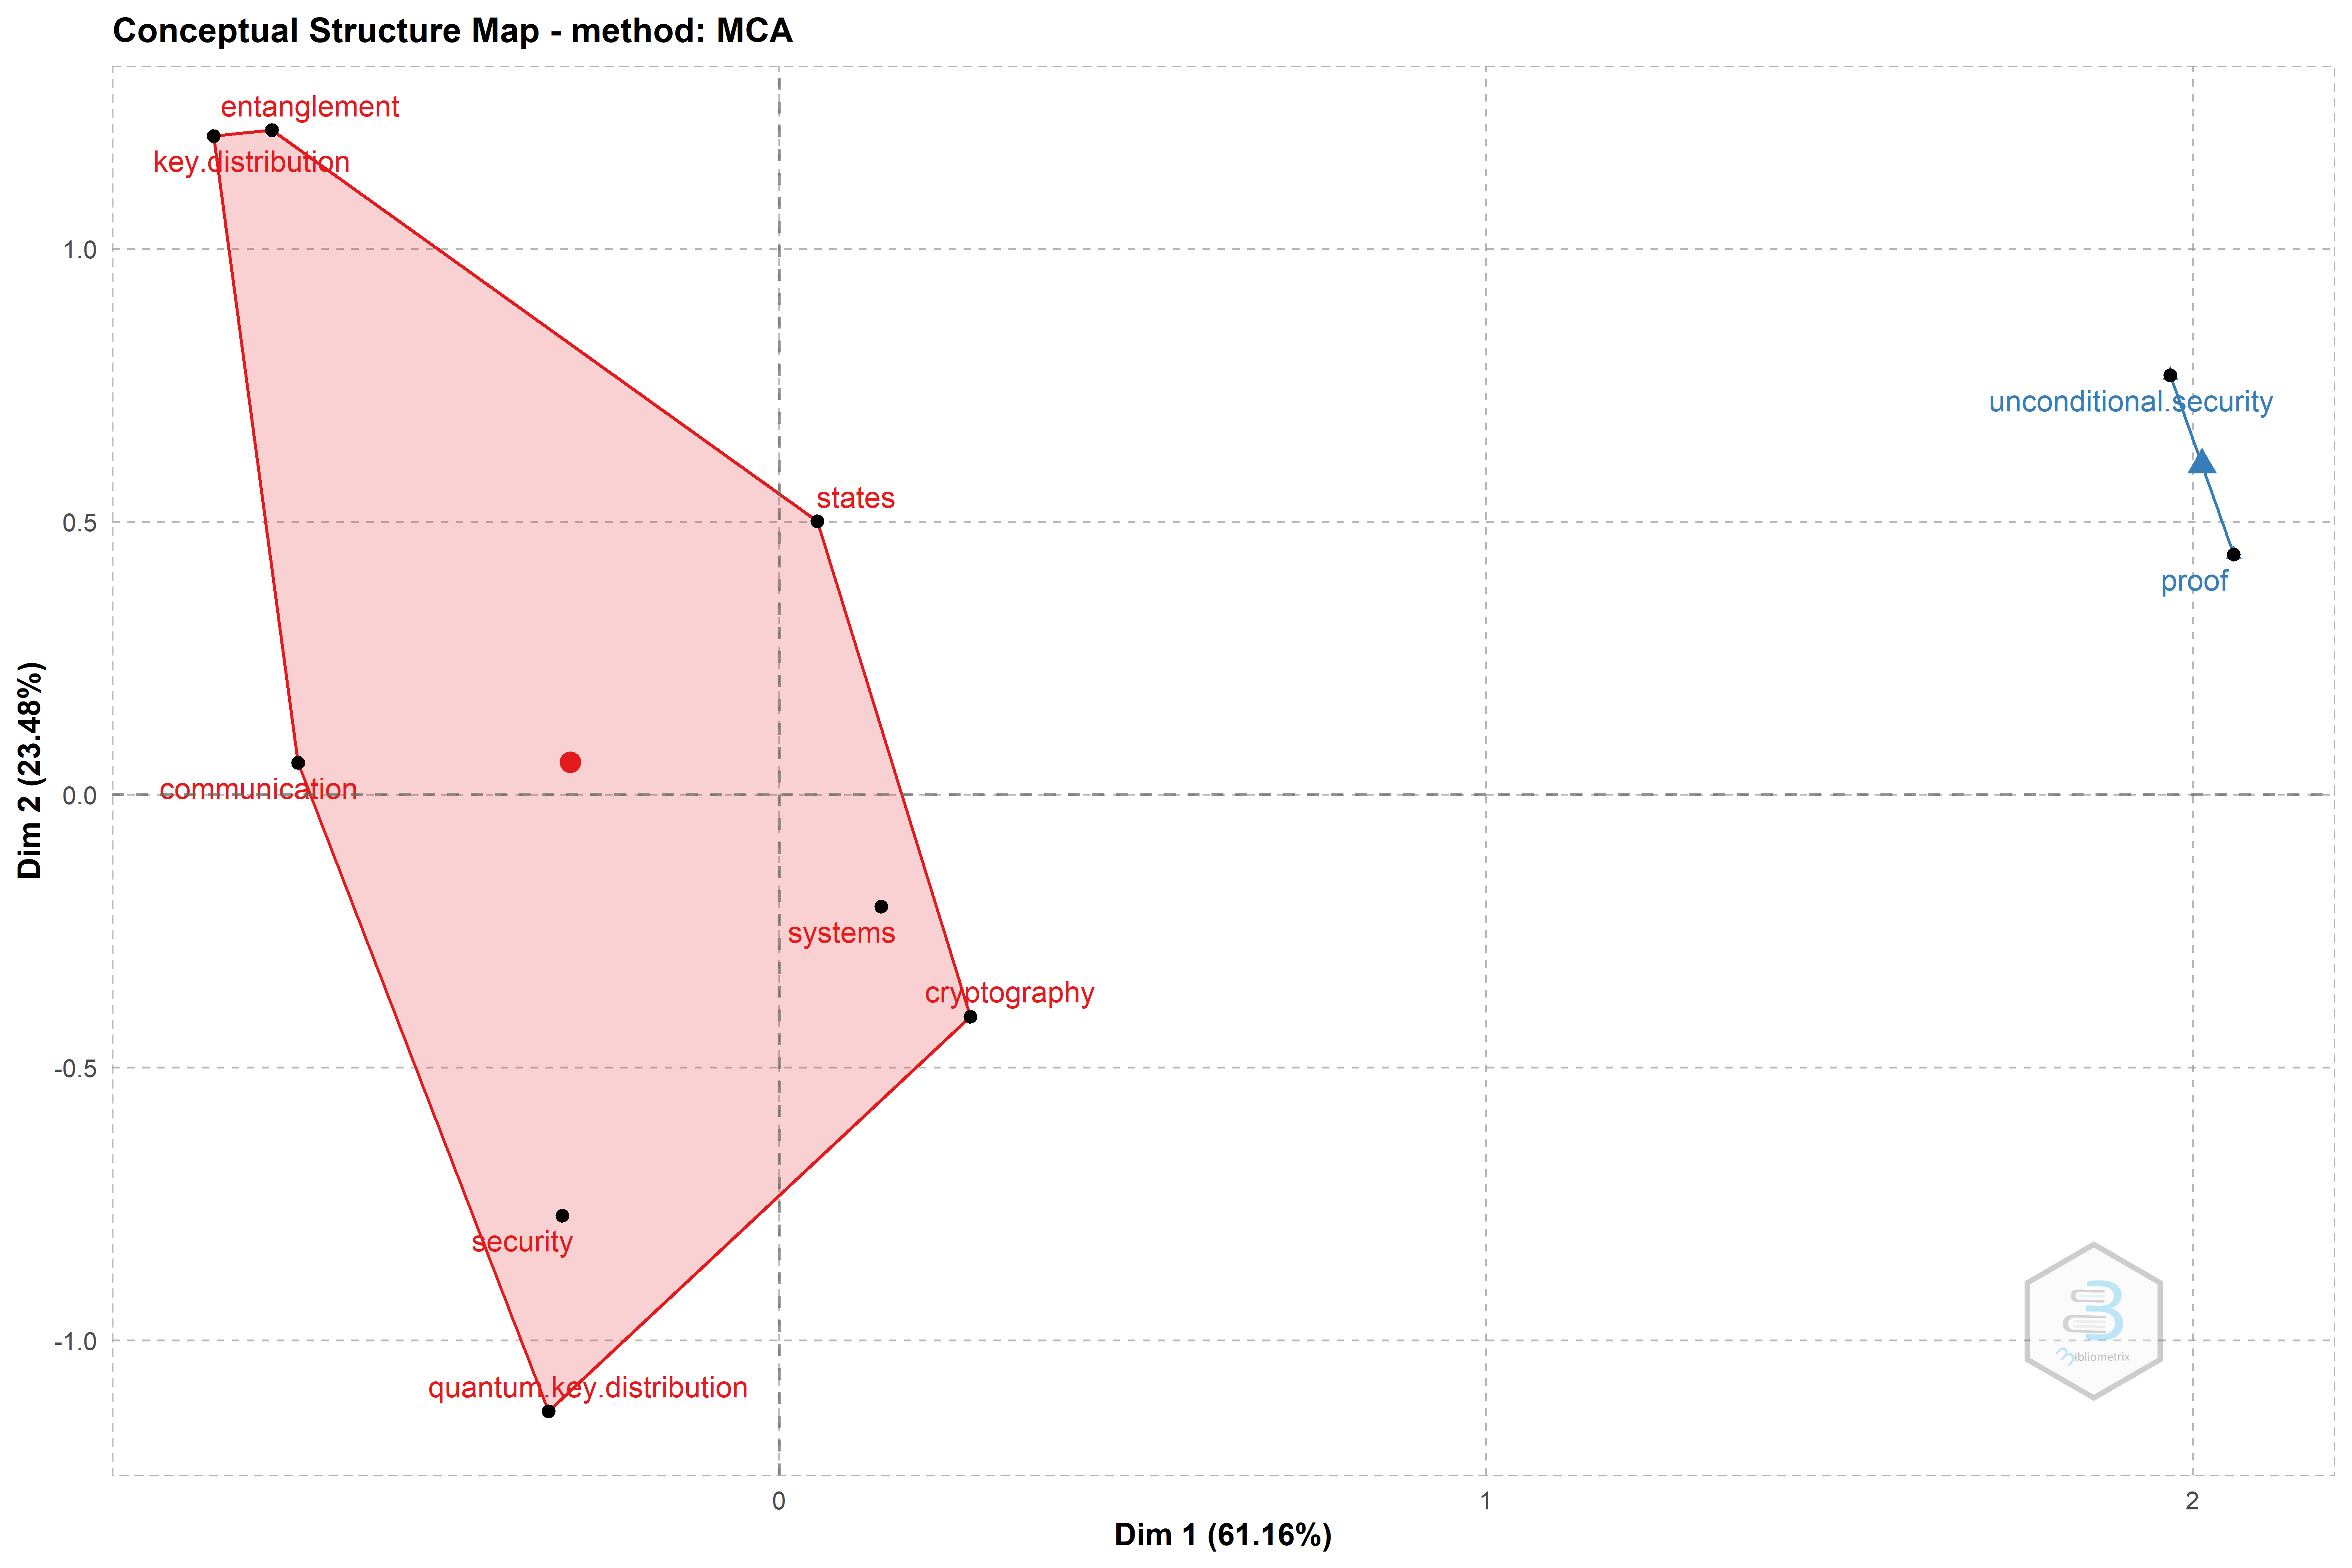
\includegraphics[width=1\textwidth]{experiments/rafaelnogalha/PesquisaBibliografica/QKDSegurancaComputacional/images/mapa_fatorial.png}
    \caption{Principais palavras-chave e o relacionamento entre si no \textit{dataset} @QKD-rafael-nogalha.}
    \label{fig:mapa:fatorial:@QKD-rafael-nogalha}
\end{figure}

\begin{figure}[H]
    \centering
    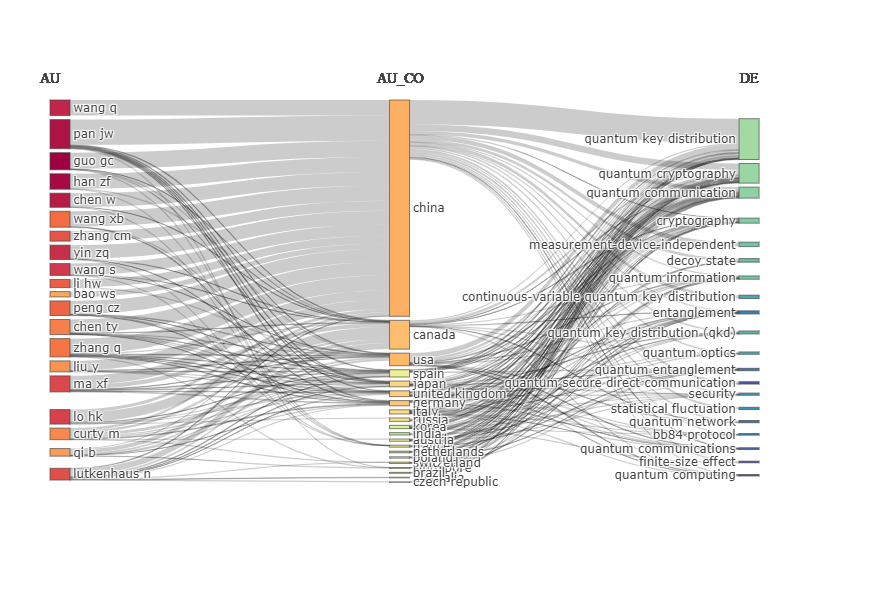
\includegraphics[width=1\textwidth]{experiments/rafaelnogalha/PesquisaBibliografica/QKDSegurancaComputacional/images/three_fields_plot_qkd.png}
    \caption{Relação entre autores, países e palavras-chave no \textit{dataset} @QKD-rafael-nogalha.}
    \label{fig:three:plot:@QKD-rafael-nogalha}
\end{figure}

\begin{figure}[H]
    \centering
    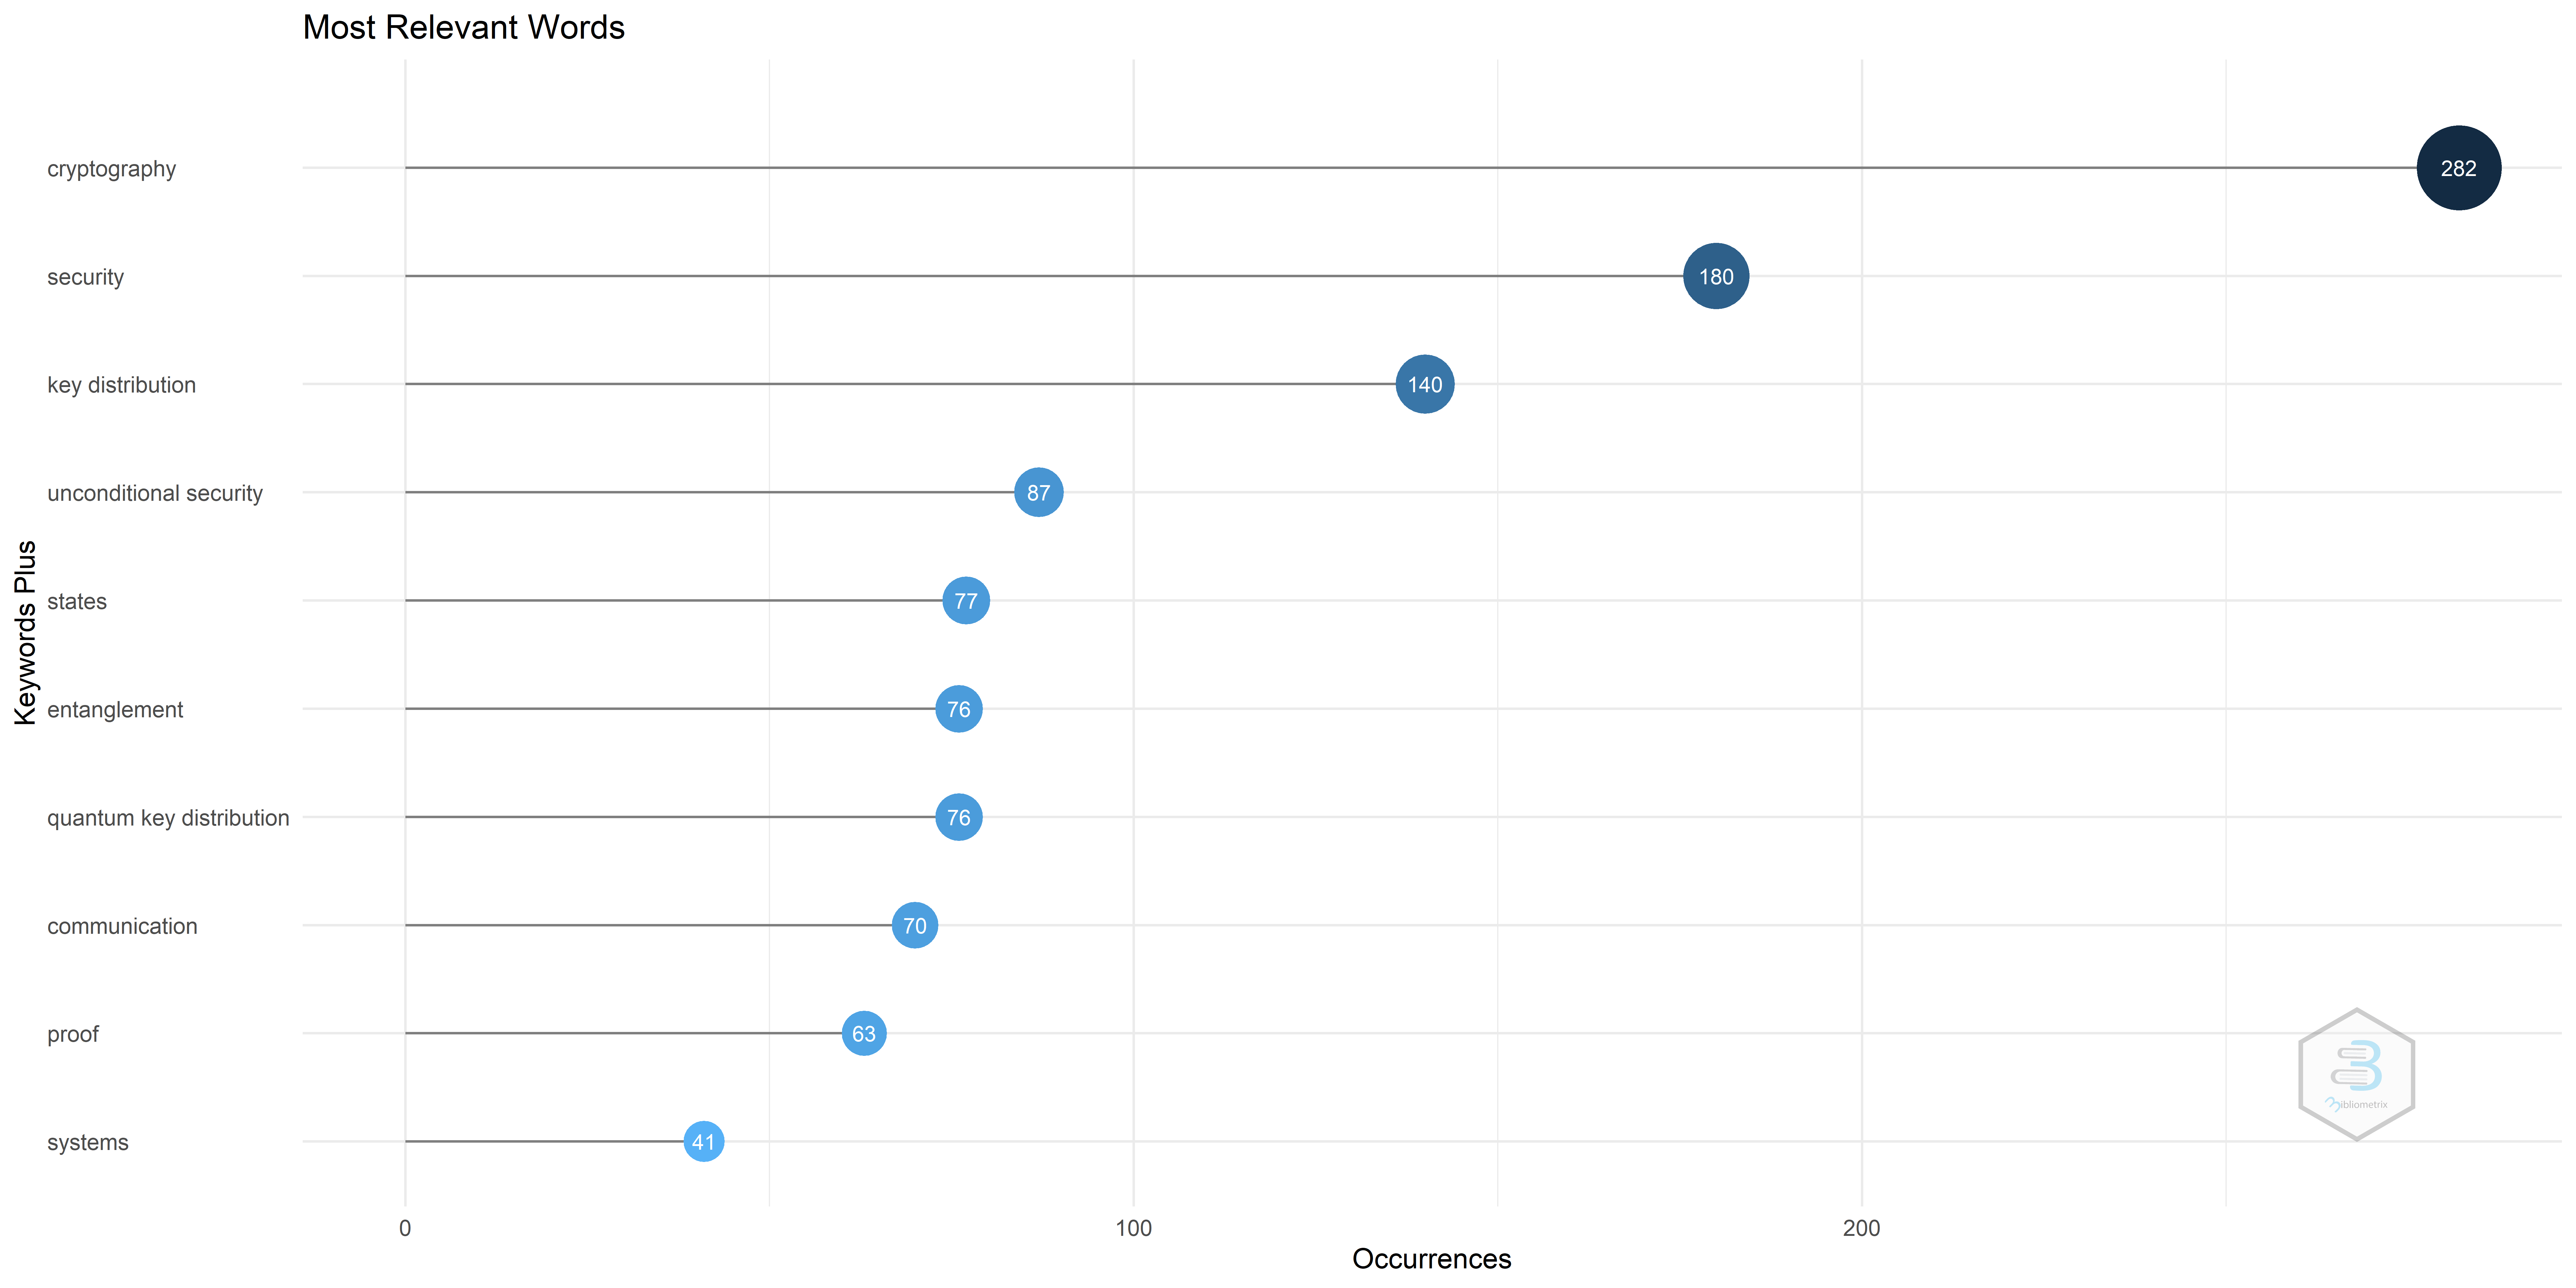
\includegraphics[width=1\textwidth]{experiments/rafaelnogalha/PesquisaBibliografica/QKDSegurancaComputacional/images/palavras_relevantes.png}
    \caption{Incidência de palavras-chave no \textit{dataset} @QKD-rafael-nogalha.}
    \label{fig:campos:plot:@QKD-rafael-nogalha}
\end{figure}



\subsection{Principais Países envolvidos e \textit{Coworking} entre ele}

Por meio das imagens abaixo, \ref{fig:map:prod:@QKD-rafael-nogalha} e \ref{fig:cowrking:prod:@QKD-rafael-nogalha}, é possível observar que a China e os Estados Unidos são os países com maior produção no presente tema do artigo e além disso são também os dois países que mais produzem materiais juntos em relação ao tema de QKD na segurança computacional. É importante ressaltar que a interação entre os países acerca do tema é forte e apresenta tendência de crescimento.

\begin{figure}[H]
    \centering
    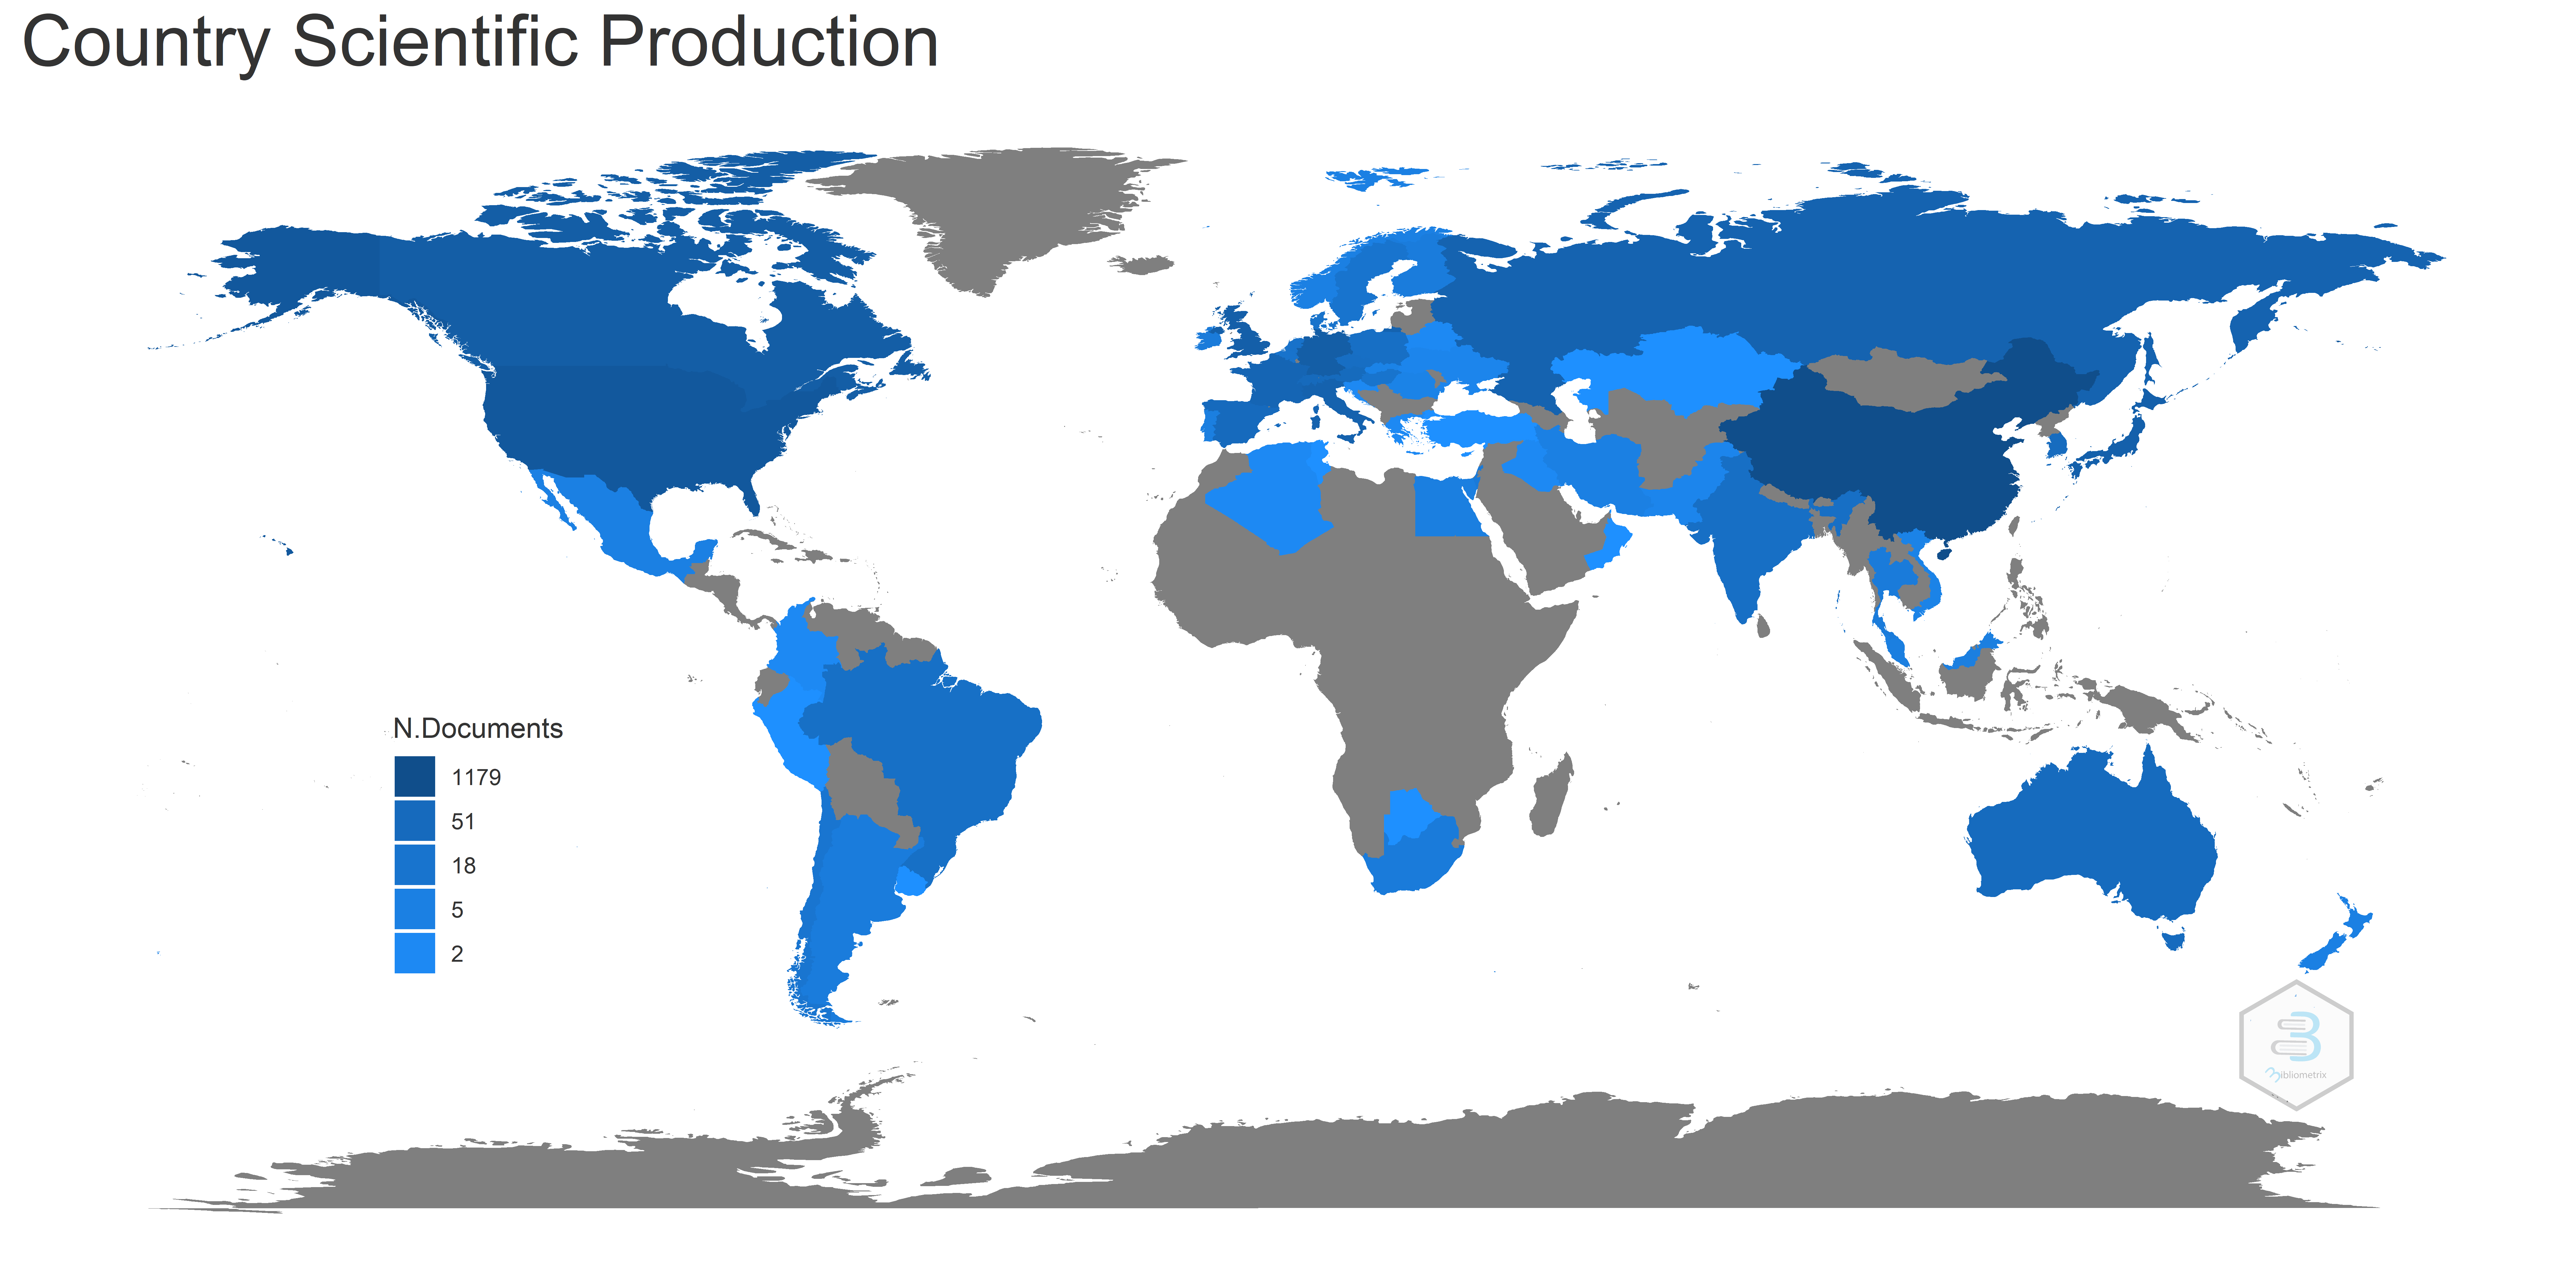
\includegraphics[width=1\textwidth]{experiments/rafaelnogalha/PesquisaBibliografica/QKDSegurancaComputacional/images/especificacao_paises_producao.png}
    \caption{Principais países que produziram artigos no \textit{dataset} @QKD-rafael-nogalha.}
    \label{fig:map:prod:@QKD-rafael-nogalha}
\end{figure}

\begin{figure}[H]
    \centering
    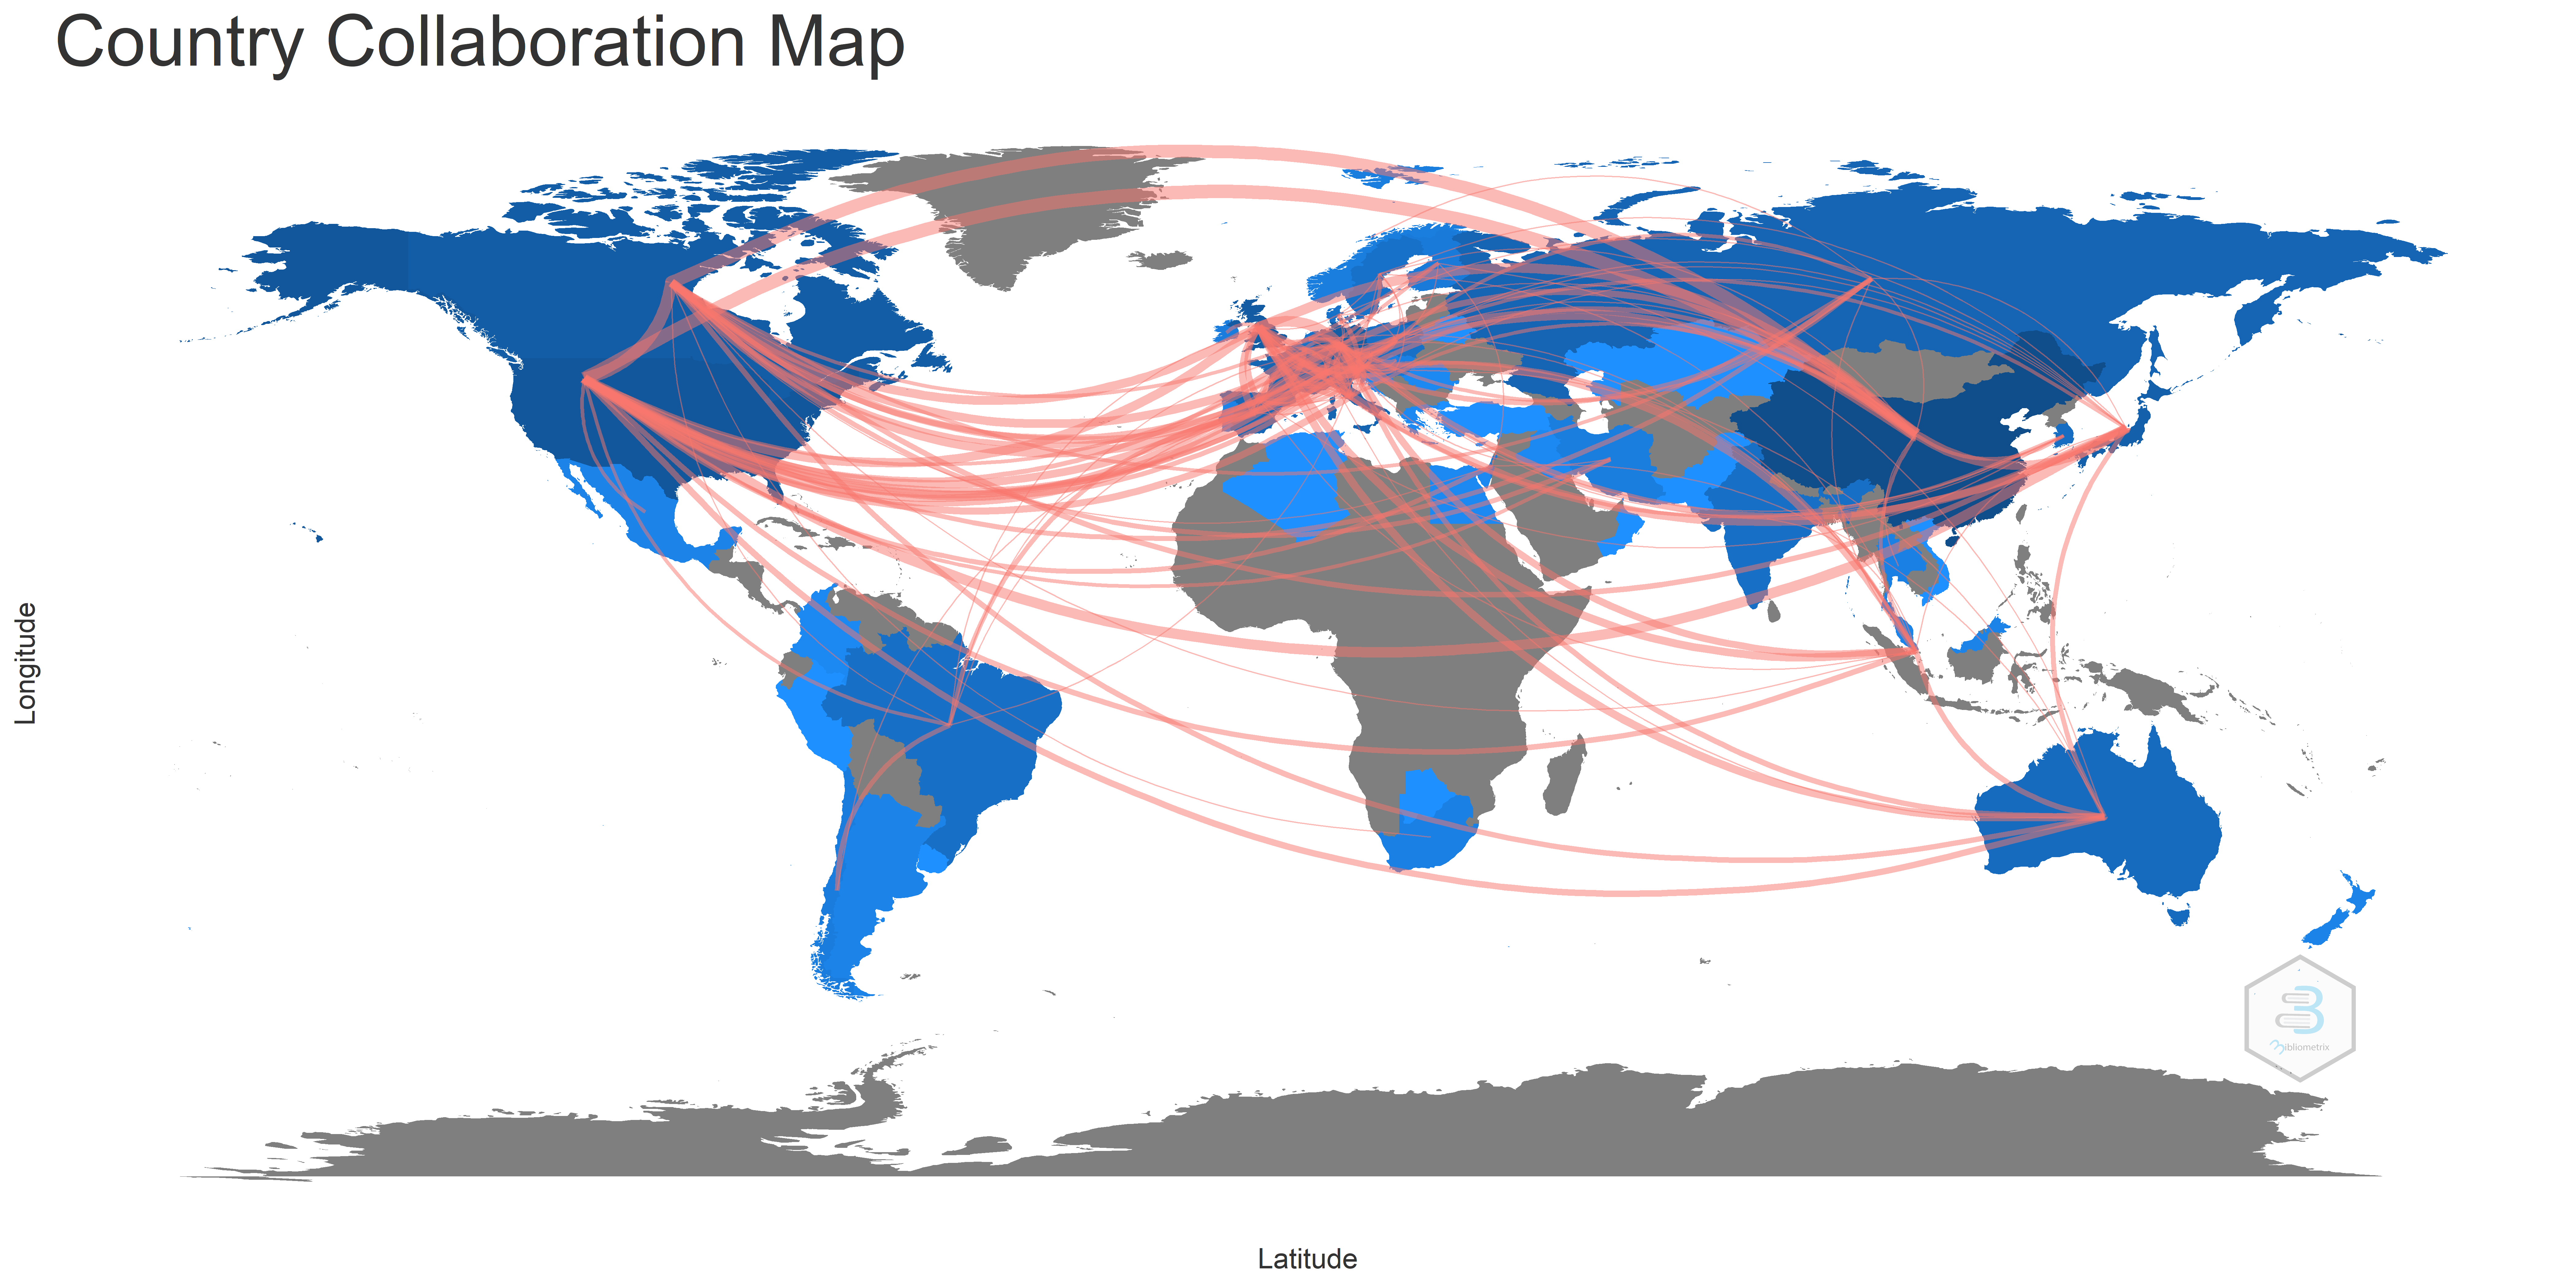
\includegraphics[width=1\textwidth]{experiments/rafaelnogalha/PesquisaBibliografica/QKDSegurancaComputacional/images/country_collaboration_map.png}
    \caption{Coworking entre os países no \textit{dataset} @QKD-rafael-nogalha.}
    \label{fig:cowrking:prod:@QKD-rafael-nogalha}
\end{figure}



\section{Resultados e interpretação}

Por meio desta pesquisa bibliográfica é possível afirmar que a produção científica em relação ao uso de \textit{QKD na Segurança Computacional} apresenta uma tendência de crescimento, além de também estar sendo compartilhada pesquisas sobre o tema em diferentes países, principalmente entre Estados Unidos e China. Por fim, é necessária uma análise mais profunda do tema para compreender melhor o uso de QKD na segurança computacional na década atual, e se será possível o uso desta teclnologia a médio ou longo prazo no mercado.